%%
%% Copyright 2007, 2008, 2009 Elsevier Ltd
%%
%% This file is part of the 'Elsarticle Bundle'.
%% ---------------------------------------------
%%
%% It may be distributed under the conditions of the LaTeX Project Public
%% License, either version 1.2 of this license or (at your option) any
%% later version.  The latest version of this license is in
%%    http://www.latex-project.org/lppl.txt
%% and version 1.2 or later is part of all distributions of LaTeX
%% version 1999/12/01 or later.
%%
%% The list of all files belonging to the 'Elsarticle Bundle' is
%% given in the file `manifest.txt'.
%%

%% Template article for Elsevier's document class `elsarticle'
%% with numbered style bibliographic references
%% SP 2008/03/01
%%
%%
%%
%% $Id: elsarticle-template-num.tex 4 2009-10-24 08:22:58Z rishi $
%%
%%
\documentclass[12pt]{elsarticle}

%% Use the option review to obtain double line spacing
%% \documentclass[preprint,review,12pt]{elsarticle}

%% Use the options 1p,twocolumn; 3p; 3p,twocolumn; 5p; or 5p,twocolumn
%% for a journal layout:
%% \documentclass[final,1p,times]{elsarticle}
%% \documentclass[final,1p,times,twocolumn]{elsarticle}
%% \documentclass[final,3p,times]{elsarticle}
%% \documentclass[final,3p,times,twocolumn]{elsarticle}
%% \documentclass[final,5p,times]{elsarticle}
%% \documentclass[final,5p,times,twocolumn]{elsarticle}

%% if you use PostScript figures in your article
%% use the graphics package for simple commands
%% \usepackage{graphics}
%% or use the graphicx package for more complicated commands
\usepackage{graphicx}
\usepackage{float}
%% or use the epsfig package if you prefer to use the old commands
%% \usepackage{epsfig}

%% The amssymb package provides various useful mathematical symbols
%\usepackage{amssymb}
%% The amsthm package provides extended theorem environments
%% \usepackage{amsthm}

%% The lineno packages adds line numbers. Start line numbering with
%% \begin{linenumbers}, end it with \end{linenumbers}. Or switch it on
%% for the whole article with \linenumbers after \end{frontmatter}.
%% \usepackage{lineno}

%% natbib.sty is loaded by default. However, natbib options can be
%% provided with \biboptions{...} command. Following options are
%% valid:

%%   round  -  round parentheses are used (default)
%%   square -  square brackets are used   [option]
%%   curly  -  curly braces are used      {option}
%%   angle  -  angle brackets are used    <option>
%%   semicolon  -  multiple citations separated by semi-colon
%%   colon  - same as semicolon, an earlier confusion
%%   comma  -  separated by comma
%%   numbers-  selects numerical citations
%%   super  -  numerical citations as superscripts
%%   sort   -  sorts multiple citations according to order in ref. list
%%   sort&compress   -  like sort, but also compresses numerical citations
%%   compress - compresses without sorting
%%
%% \biboptions{comma,round}

% \biboptions{}

\journal{Computational and Applied Mathematics}

\begin{document}

\begin{frontmatter}

%% Title, authors and addresses

%% use the tnoteref command within \title for footnotes;
%% use the tnotetext command for the associated footnote;
%% use the fnref command within \author or \address for footnotes;
%% use the fntext command for the associated footnote;
%% use the corref command within \author for corresponding author footnotes;
%% use the cortext command for the associated footnote;
%% use the ead command for the email address,
%% and the form \ead[url] for the home page:
%%

\title{Solving a Suite of NIST Benchmark Problems\\ for Adaptive FEM with the Hermes Library}

%% use optional labels to link authors explicitly to addresses:
\author[label1]{Zhonghua Ma}
\ead{mazhonghua83@gmail.com}
\author[label2]{Lukas Korous}
\ead{lukas.korous@gmail.com}
\author[label3]{Erick Santiago}
\ead{laviticus@sbcglobal.net}
\address[label1]{China University of Petroleum, Beijing, China}
\address[label2]{Charles University, Prague, Czech Republic}
\address[label3]{University of Nevada, Reno, USA}

\begin{abstract}
Recently, a new suite of twelve benchmark problems for adaptive finite element methods (FEM)
was published at the U.S. National Institute for Standards and Technology (NIST).
These test problems come with exact solutions, and they exhibit all typical difficulties
associated with elliptic problems including singularities, steep internal layers, anisotropy,
and oscillations. In this paper we solve these benchmark problems using the open source
library Hermes (http://hpfem.org). All these results are reproducible -- they are part of
the Git repository of the open source Hermes project, and the reader can experiment
with them by himself/herself. Instructions for this are provided. We hope that authors
of other adaptive FEM codes will make their results for these test problems available
in a reproducible fashion as well.
\end{abstract}

\begin{keyword}
finite element method \sep automatic adaptivity \sep benchmark problem \sep reproducible research
%% keywords here, in the form: keyword \sep keyword
%% MSC codes here, in the form: \MSC code \sep code
%% or \MSC[2008] code \sep code (2000 is the default)
\end{keyword}

\end{frontmatter}

%% main text
\section{Introduction}
\label{sec:intro}

The number of adaptive finite element (FEM) codes is growing very fast.
They differ in deployment operating systems and hardware platforms,
ways of loading the physical model, error estimation mechanisms,
algebraic solvers they use, mesh formats, boundary conditions
handling, input/output formats, and other aspects. Some of them are
designed for a narrow class of problems while others are supposed to
cover various types of physical applications. In summary, these facts
make it extremely difficult to assess and compare the accuracy and
performance of various adaptive FEM codes.

Recently, Dr. William Mitchell (NIST) collected a suite of
twelve benchmark problems with known exact solution for adaptive
FEM \cite{mitchell-1}. The advantage of having an exact solution is that
the approximation error can be calculated very accurately, thus
enabling fair comparison of results calculated with different
programs. All these examples are elliptic, and they are defined
in very simple geometries, to make their solution possible with
virtually any FEM code.

In this paper, we solve the twelve benchmarks using
Hermes, a multi-platform open source C++
library for rapid development of adaptive $hp$-FEM
and $hp$-DG solvers (http://hpfem.org). A few words
and links to the Hermes library will be presented at the
end of the paper, but only very briefly, as this is not
the major objective of the paper. Our main goal is to
respond to \cite{mitchell-1} by providing results by
the Hermes library, and make them easily reproducible
for anyone.

To make the paper reasonably self-contained, we must repeat some
material from \cite{mitchell-1}, but this is done in a minimalistic way.
Each of the following sections contains a short description of
the benchmark problem followed by results and convergence graphs in terms of degrees
of freedom (DOF) and CPU time. Conclusion and outlook
is presented at the end of the paper.

%%%%%%%%%%%%%%%%%%%%%%%%%%%%%%%%%%%%%%%%%%%%

\section{Benchmark NIST-1 "Analytic Solution"}
\label{sec:bench-1}

This benchmark problem has a smooth solution.
Solved is the Poisson equation

\begin{equation} \label{poisson}
-\Delta u = f
\end{equation}
in the domain $\Omega = (0, 1)^2$, equipped with Dirichlet
boundary condition given by the exact solution.
The exact solution is $u(x, y) = 2^{4p}x^{p}(1-x)^{p}y^{p}(1-y)^{p}$
with $p = 10$.
The solution to NIST-1 is shown in Fig. \ref{fig:sln-nist01}.

\begin{figure}[H]
\centering
%\vspace{-3mm}
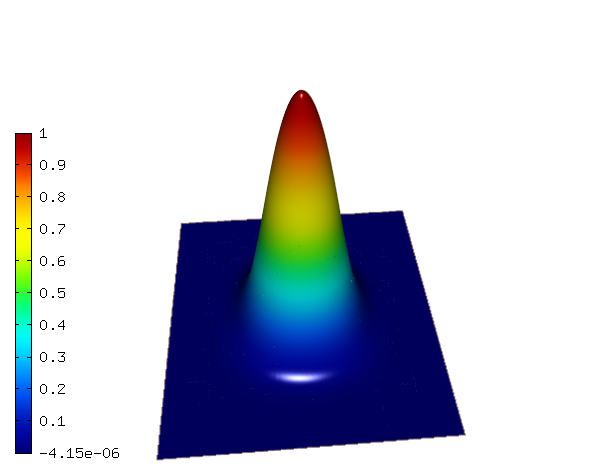
\includegraphics[height=5cm]{nist/nist-1/solution.png}
%\vspace{-3mm}
\caption{Solution to the NIST-1 benchmark problem.}
\label{fig:sln-nist01}
\end{figure}

Fig. \ref{fig:nist-1-hp-aniso} presents the final meshes corresponding to adaptive $h$-FEM with
linear elements, adaptive $h$-FEM with quadratic elements, and adaptive $hp$-FEM. Different
polynomial degrees of elements are represented by different colors.

\begin{figure}[!ht]
\centering
%\vspace{-7mm}
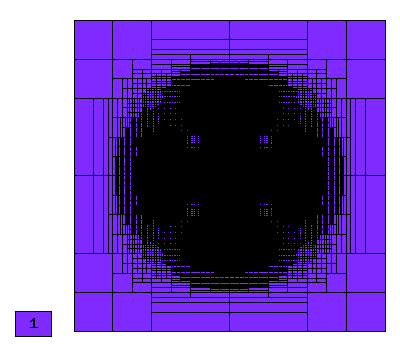
\includegraphics[height=3.7cm]{nist/nist-1/mesh_h1_aniso.png}
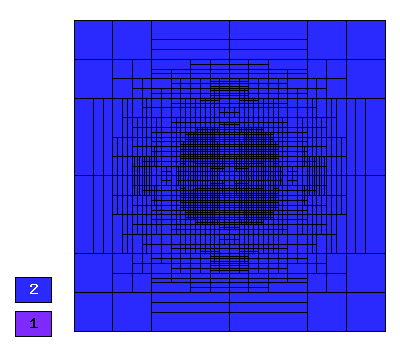
\includegraphics[height=3.7cm]{nist/nist-1/mesh_h2_aniso.png}
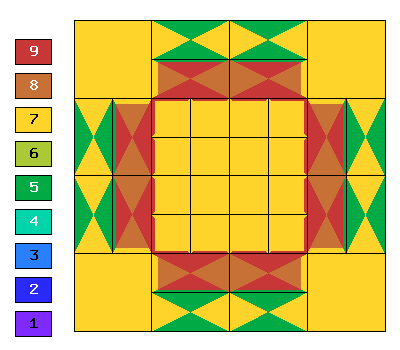
\includegraphics[height=3.7cm]{nist/nist-1/mesh_hp_aniso.png}
%\vspace{-3mm}
\caption{
Left: Final mesh with 51365 DOF and relative error 5.87223e-01~\% for $h$-FEM with linear elements.
Middle: Final mesh with 43401 DOF and relative error 1.37127e-02~\% for $h$-FEM with quadratic elements.
Right: Final mesh with 1325 DOF and relative error 9.34911e-04~\% for $hp$-FEM (adaptivity option HP\_ANISO).}
\label{fig:nist-1-hp-aniso}
%\vspace{-3mm}
\end{figure}

Fig. \ref{fig:nist-1-conv} shows the convergence of the adaptive methods in terms of DOF and CPU-time.

\begin{figure}[H]
\centering
%\vspace{-3mm}
\hspace{-50mm}
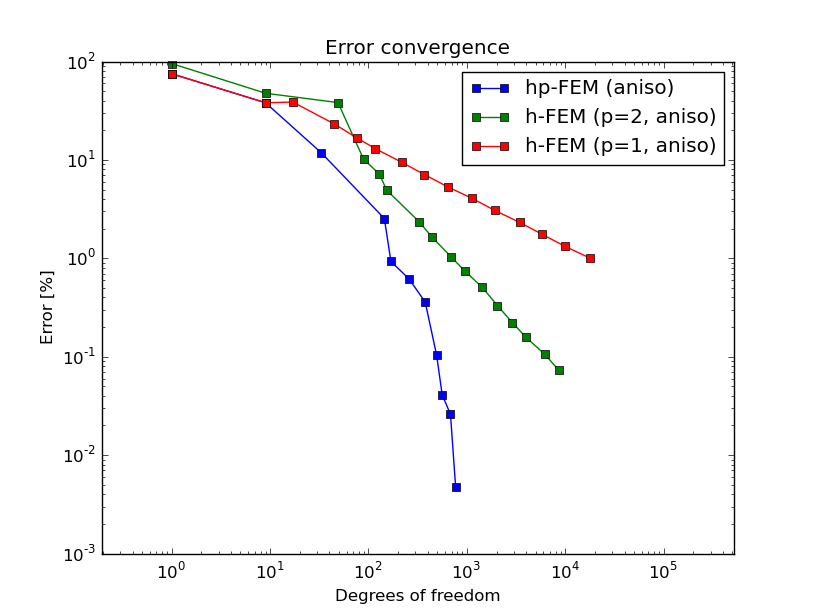
\includegraphics[width=7.5cm]{nist/nist-1/conv_dof_aniso.png}\ \
\hspace{-8mm}
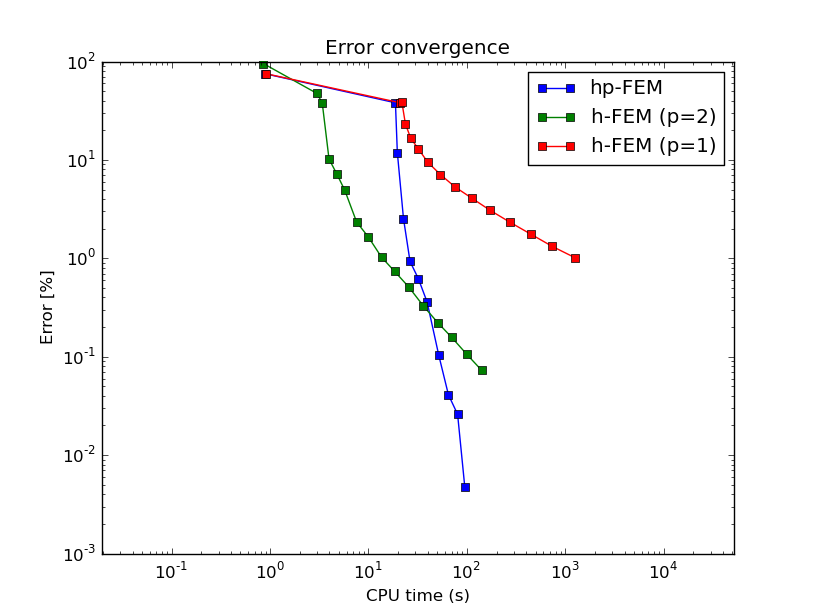
\includegraphics[width=7.5cm]{nist/nist-1/conv_cpu_aniso.png}
\hspace{-50mm}
\vspace{-2mm}
\caption{DOF and CPU time convergence graphs.}
%\vspace{-1mm}
\label{fig:nist-1-conv}
\end{figure}

%%%%%%%%%%%%%%%%%%%%%%%%%%%%%%%%%%%%%%%%%%%%%%%%%%

\section{Benchmark NIST-2 "Reentrant Corner"}
\label{sec:bench-2}

The exact solution of this problem is smooth but it contains
singular gradient at the reentrant corner.
Solved is the Laplace equation

\begin{equation} \label{laplace}
-\Delta u = 0
\end{equation}
in the domain $\Omega = (-1, 1)^2$, with a unit square
section removed from the bottom part of the positive $x$ axis.
Equation (\ref{laplace}) equipped with Dirichlet
boundary conditions given by the exact solution
$u(x, y) = r^{\alpha}\sin(\alpha \theta)$,
where $\alpha = \pi / \omega$, $r = \sqrt{x^2+y^2}$,
and $\theta = tan^{-1}(y/x)$. Here $\omega $ determines
the angle of the reentrant corner.
The solution to NIST-2 with $\omega = 3 \pi / 2$
is shown in Fig. \ref{fig:sln-nist02}.

\begin{figure}[H]
\centering
\vspace{-1mm}
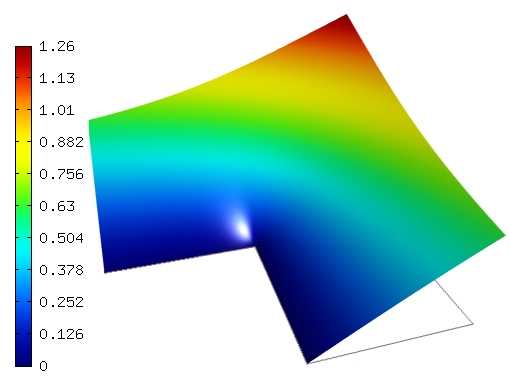
\includegraphics[height=5cm]{nist/nist-2/solution.png}
\vspace{-1mm}
\caption{Solution to the NIST-2 benchmark problem.}
\label{fig:sln-nist02}
\end{figure}

Fig. \ref{fig:nist-2-hp-aniso} presents the final meshes corresponding to adaptive $h$-FEM with
linear elements, adaptive $h$-FEM with quadratic elements, and adaptive $hp$-FEM. Different
polynomial degrees of elements are represented by different colors.

\begin{figure}[H]
\centering
\vspace{-2mm}
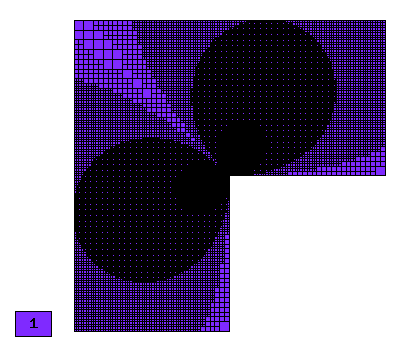
\includegraphics[height=3.7cm]{nist/nist-2/mesh_h1_aniso.png}
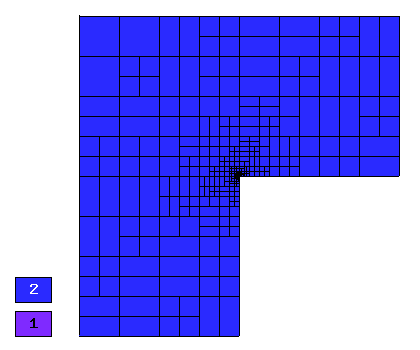
\includegraphics[height=3.7cm]{nist/nist-2/mesh_h2_aniso.png}
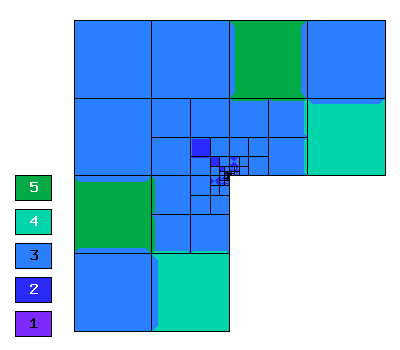
\includegraphics[height=3.7cm]{nist/nist-2/mesh_hp_aniso.png}
\vspace{-2mm}
\caption{
Left: Final mesh with 46097 DOF and relative error 1.30193e-01~\% for $h$-FEM with linear elements.
Middle: Final mesh with 59049 DOF and relative error 1.65778e-03~\% for $h$-FEM with quadratic elements.
Right: Final mesh with 2756 DOF and relative error 9.78935e-04~\% for $hp$-FEM (adaptivity option HP\_ANISO\_H).}
\label{fig:nist-2-hp-aniso}
\vspace{-2mm}
\end{figure}

Fig. \ref{fig:nist-2-conv} shows the convergence of the adaptive methods in terms of DOF and CPU-time.

\begin{figure}[H]
\centering
\vspace{-3mm}
\hspace{-50mm}
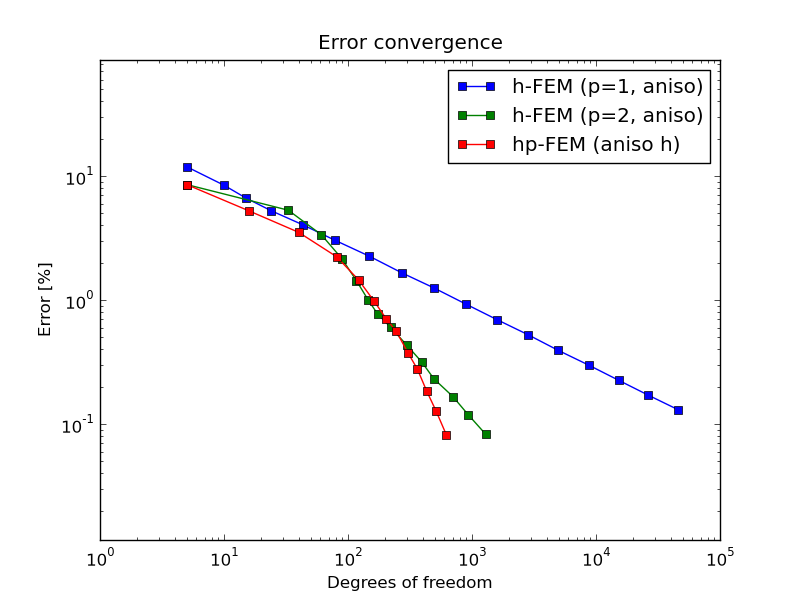
\includegraphics[width=7.5cm]{nist/nist-2/conv_dof_aniso.png}\ \
\hspace{-10mm}
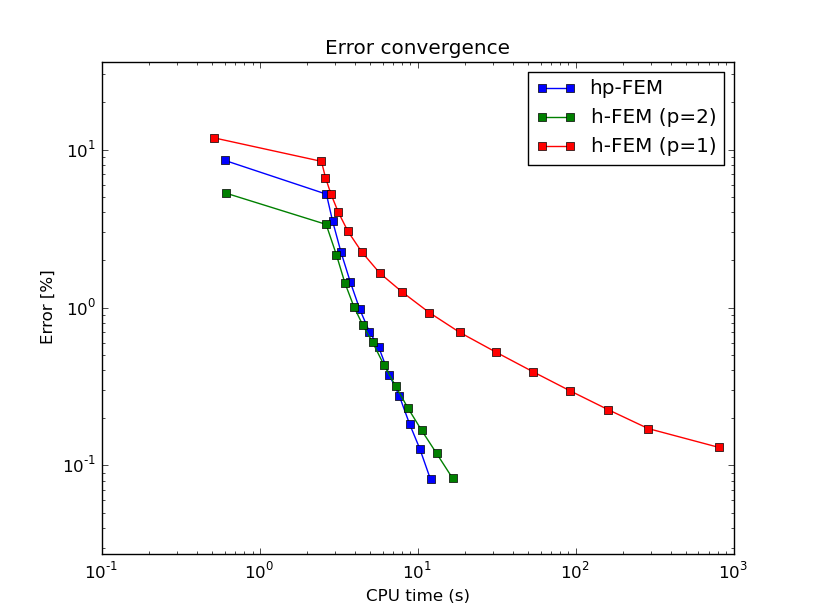
\includegraphics[width=7.5cm]{nist/nist-2/conv_cpu_aniso.png}
\hspace{-50mm}
\vspace{-2mm}
\caption{DOF and CPU time convergence graphs.}
\label{fig:nist-2-conv}
\end{figure}

%%%%%%%%%%%%%%%%%%%%%%%%%%%%%%%%%%%%%%%%%%%%%%%%%%%%%%%

\section{Benchmark NIST-3 "Linear Elasticity"}
\label{sec:bench-3}

This benchmark deals with the Lam\'e equations of linear elasticity.
Since the two resulting displacement components $u, v$ are very different, we use the
multimesh functionality of Hermes \cite{label2,thermoel} which makes it
possible to approximate them on different meshes that moreover
are locally refined independently of each other.
The equations have the form
\vspace{-3mm}

\begin{equation}\label{crack}
\left\{
\begin{array}{l}
\displaystyle
-E \frac{1-\nu^2}{1-2\nu} \frac{\partial^{2} u}{\partial x^{2}} - E\frac{1-\nu^2}{2-2 \nu} \frac{\partial^{2} u}{\partial y^{2}}
-E \frac{1-\nu^2}{(1-2\nu)(2-2\nu)} \frac{\partial^{2} v}{\partial x \partial y} = 0, \\[3mm]
\displaystyle
-E \frac{1-\nu^2}{2-2\nu} \frac{\partial^{2} v}{\partial x^{2}} - E\frac{1-\nu^2}{1-2\nu} \frac{\partial^{2} v}{\partial y^{2}}
-E \frac{1-\nu^2}{(1-2\nu)(2-2\nu)} \frac{\partial^{2} u}{\partial x \partial y} = 0,
\end{array}
\right.
\end{equation}
where $u$ and $v$ are the
$x$ and $y$ displacements, $E$ is Young's Modulus,
and $\nu$ is Poisson ratio.
The domain in the example is $\Omega = (-1, 1)^2$ with a slit $([0,0], [1,0])$,
equipped with Dirichlet boundary conditions given by the
exact solution in polar coordinates as

\[
\left\{
\begin{array}{l}
\displaystyle
u(x, y) = \frac{1}{2G} r^{\lambda}[(k - Q(\lambda + 1))cos(\lambda \theta) - \lambda cos((\lambda - 2) \theta)],  \\[3mm]
\displaystyle
v(x, y) = \frac{1}{2G} r^{\lambda}[(k + Q(\lambda + 1))sin(\lambda \theta) + \lambda sin((\lambda - 2) \theta)],
\end{array}
\right.
\]
where $\lambda = 0.5444837367825$, $Q = 0.5430755788367$,
$k = 3 - 4 \nu$ and $G = E / (2(1 + \nu))$.
The solution to NIST-3 is shown in Fig. \ref{fig:sln-nist03}.
%\vspace{-4mm}

\begin{figure}[H]
\centering
%\vspace{-1mm}
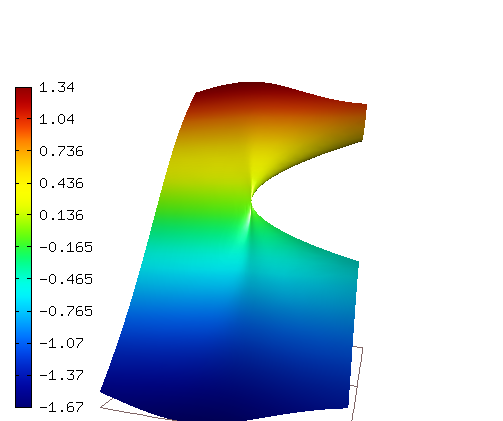
\includegraphics[height=5cm]{nist/nist-3/solution-u.png}\ \
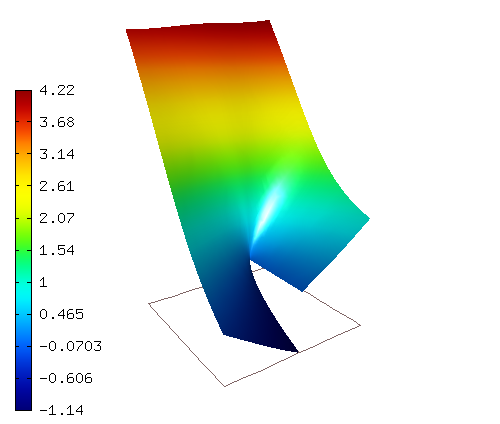
\includegraphics[height=5cm]{nist/nist-3/solution-v.png}
%\vspace{-1mm}
\caption{The $u$ (left) and $v$ (right) component to NIST-3 benchmark problem.}
%\vspace{-3mm}
\label{fig:sln-nist03}
\end{figure}

Fig. \ref{fig:nist-3-hp-aniso} presents the final meshes corresponding to adaptive $h$-FEM with
linear elements, adaptive $h$-FEM with quadratic elements, and adaptive $hp$-FEM. Different
polynomial degrees of elements are represented by different colors.

\begin{figure}[!ht]
\centering
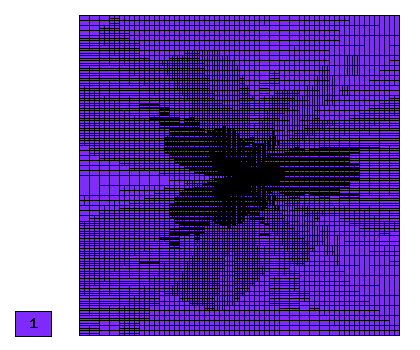
\includegraphics[height=3.7cm]{nist/nist-3/mesh_u_h1_aniso.png}
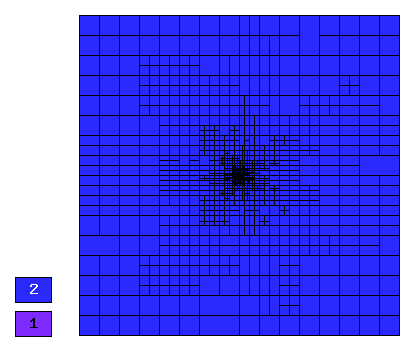
\includegraphics[height=3.7cm]{nist/nist-3/mesh_u_h2_aniso.png}
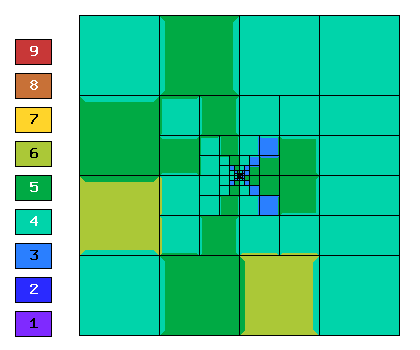
\includegraphics[height=3.7cm]{nist/nist-3/mesh_u_hp_anisoh.png}\ \
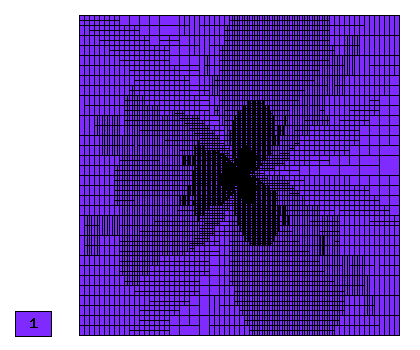
\includegraphics[height=3.7cm]{nist/nist-3/mesh_v_h1_aniso.png}
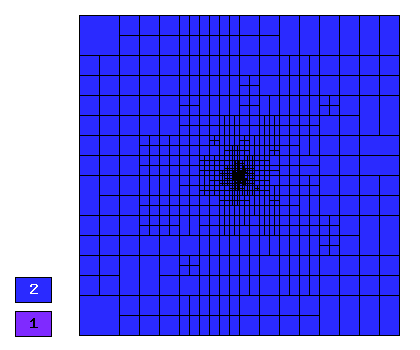
\includegraphics[height=3.7cm]{nist/nist-3/mesh_v_h2_aniso.png}
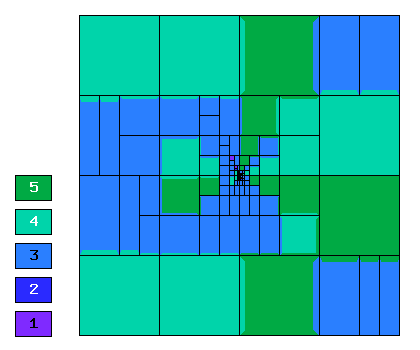
\includegraphics[height=3.7cm]{nist/nist-3/mesh_v_hp_anisoh.png}
\caption{
Left: Final mesh with 39779 DOF and relative error 3.84929e-01~\% for $h$-FEM with linear elements.
Middle: Final mesh with 9330 DOF and relative error 9.56383e-02~\% for $h$-FEM with quadratic elements.
Right: Final mesh with 3897 DOF and relative error 8.05635e-02~\% for $hp$-FEM (adaptivity option HP\_ANISO\_H).}
\label{fig:nist-3-hp-aniso}
\end{figure}

Fig. \ref{fig:nist-3-conv} shows the convergence of the adaptive methods in terms of DOF and CPU-time.

\begin{figure}[H]
\centering
\hspace{-50mm}
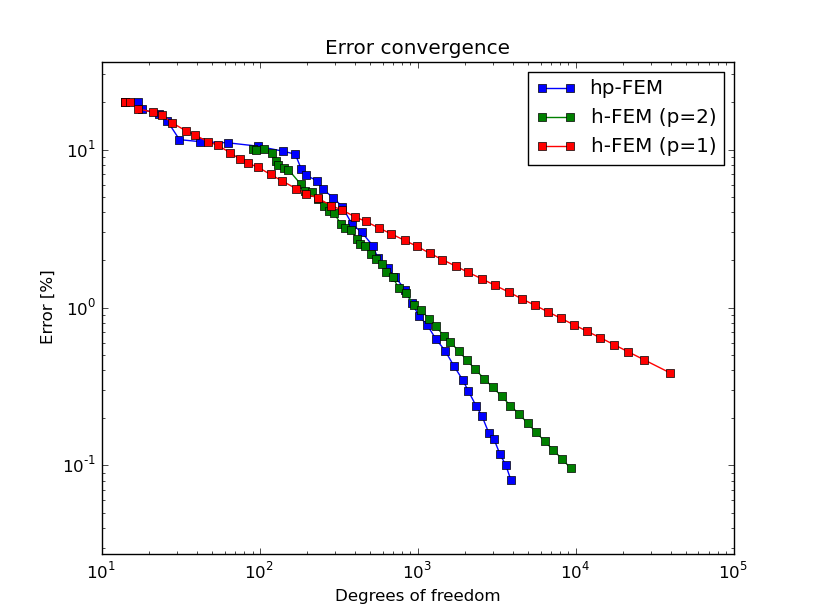
\includegraphics[width=7.5cm]{nist/nist-3/conv_dof_aniso.png}\ \
\hspace{-10mm}
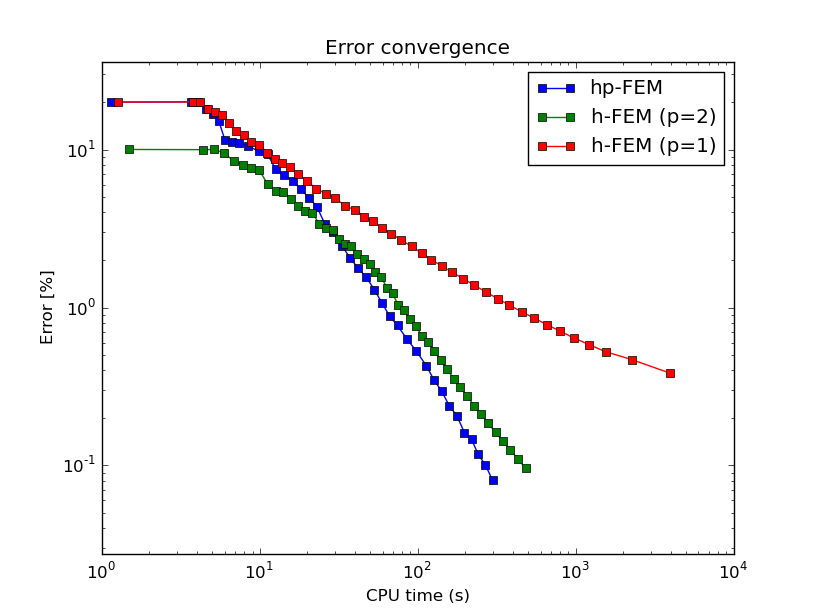
\includegraphics[width=7.5cm]{nist/nist-3/conv_cpu_aniso.png}
\hspace{-50mm}
\vspace{-2mm}
\caption{DOF and CPU time convergence graphs.}
\label{fig:nist-3-conv}
\end{figure}

%%%%%%%%%%%%%%%%%%%%%%%%%%%%%%%%%%%%%%%%%%%%%%%%

\section{Benchmark NIST-4 "Peak"}
\label{sec:bench-4}

The solution to this problem exhibits an exponential peak in the interior of the domain.
The equation solved in this benchmark problem is the Poisson equation.

\begin{equation} \label{poisson-peak}
-\Delta u = f
\end{equation}
in the domain $\Omega = (0, 1)^2$, equipped with Dirichlet
boundary conditions given by the exact solution.
The exact solution is
$u(x,y) = e^{-\alpha ((x - x_{loc})^{2} + (y - y_{loc})^{2})}$,
where $(x_{loc}, y_{loc})$ is the location of the peak,
and $\alpha$ determines the strength of the peak.
The solution to NIST-4 with $\alpha = 1000$,
$(x_{loc}, y_{loc}) = (0.5, 0.5)$ is shown in Fig. \ref{fig:sln-nist04}.

\begin{figure}[H]
\centering
%\vspace{-3mm}
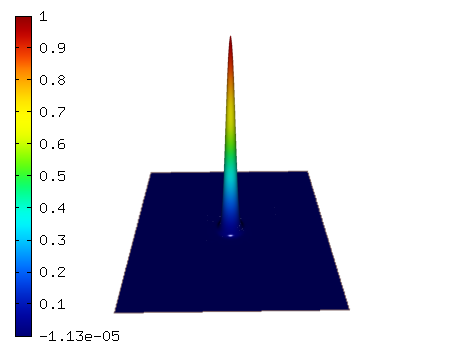
\includegraphics[height=5cm]{nist/nist-4/solution.png}
%\vspace{-3mm}
\caption{Solution to the NIST-4 benchmark problem.}
\vspace{-3mm}
\label{fig:sln-nist04}
\end{figure}

Fig. \ref{fig:nist-4-hp-aniso} presents the final meshes corresponding to adaptive $h$-FEM with
linear elements, adaptive $h$-FEM with quadratic elements, and adaptive $hp$-FEM. Different
polynomial degrees of elements are represented by different colors.

\begin{figure}[H]
\centering
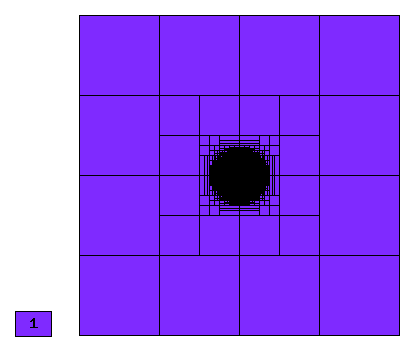
\includegraphics[height=3.7cm]{nist/nist-4/mesh_h1_aniso.png}
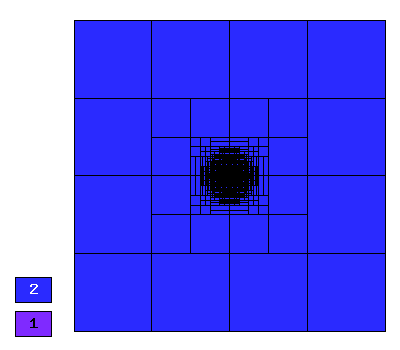
\includegraphics[height=3.7cm]{nist/nist-4/mesh_h2_aniso.png}
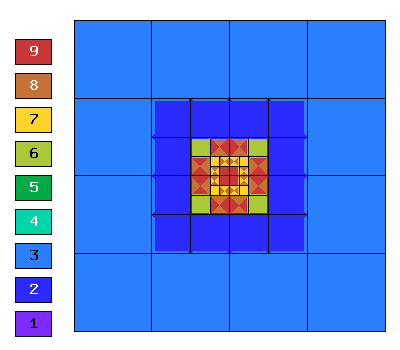
\includegraphics[height=3.7cm]{nist/nist-4/mesh_hp_aniso.png}
\caption{
Left: Final mesh with 58253 DOF and relative error 5.72234e-01~\% for $h$-FEM with linear elements.
Middle: Final mesh with 51473 DOF and relative error 1.39525e-02~\% for $h$-FEM with quadratic elements.
Right: Final mesh with 973 DOF and relative error 7.72434e-03~\% for $hp$-FEM (adaptivity option HP\_ANISO).}
\label{fig:nist-4-hp-aniso}
\end{figure}

Fig. \ref{fig:nist-4-conv} shows the convergence of the adaptive methods in terms of DOF and CPU-time.

\begin{figure}[H]
\centering
%\vspace{-4mm}
\hspace{-50mm}
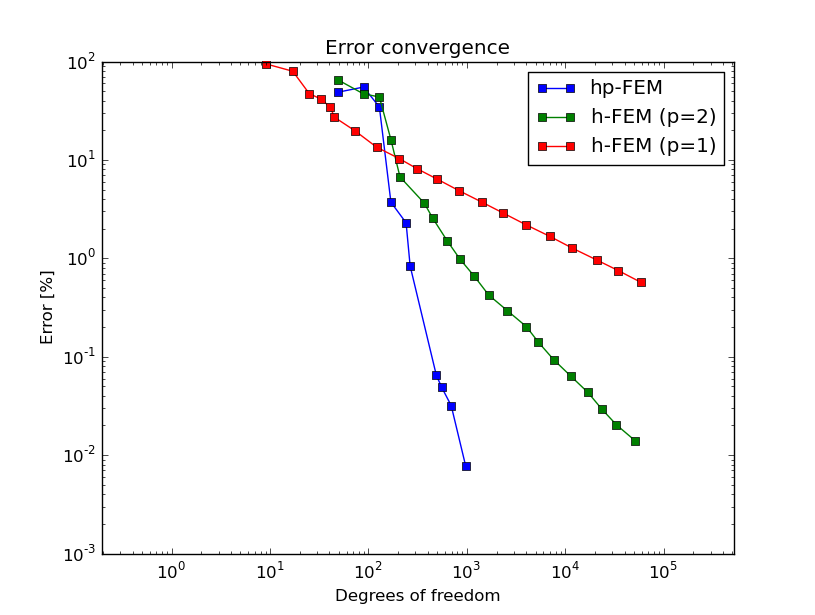
\includegraphics[width=7.5cm]{nist/nist-4/conv_dof_aniso.png}\ \
\hspace{-10mm}
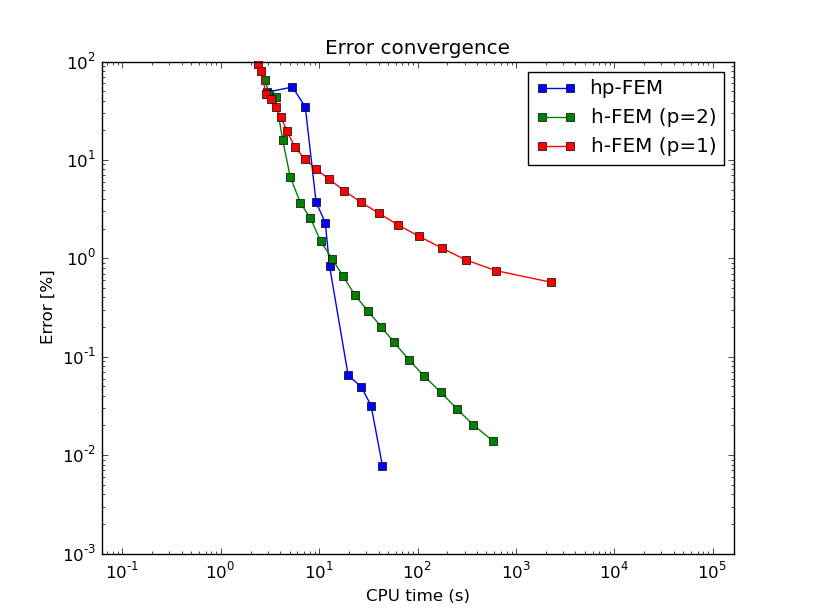
\includegraphics[width=7.5cm]{nist/nist-4/conv_cpu_aniso.png}
\hspace{-50mm}
\vspace{-2mm}
\caption{DOF and CPU time convergence graphs.}
\label{fig:nist-4-conv}
\end{figure}

%%%%%%%%%%%%%%%%%%%%%%%%%%%%%%%%%%%%%%%%%%%%%%%%

\section{Benchmark NIST-5 "Battery"}
\label{sec:bench-5}

This is a heat conduction problem in a nonhomogeneous material.
It comes with an anisotropic solution with strong internal disruption
layers and singularities.
The solution has multiple point singularities in the interior at which
more than three different materials meet. These singularities are stronger than those
corresponding to reentrant corners. The equation solved is

\begin{equation} \label{heat-conduction}
-\frac{\partial }{\partial x}\left(p(x, y)\frac{\partial u}{\partial x}\right)
-\frac{\partial }{\partial y}\left(q(x, y)\frac{\partial u}{\partial y}\right) = f
\end{equation}
in the domain $\Omega = (0, 8.4) \times (0, 24)$. Boundary conditions are zero Neumann on left edge, Newton on the rest of the boundary.
The right-hand side $f$ are constant functions (different in respective materials) given in \cite{mitchell-1}.
The solution to NIST-5 is shown in Fig. \ref{fig:sln-nist05}.

\begin{figure}[H]
\centering
%\vspace{-3mm}
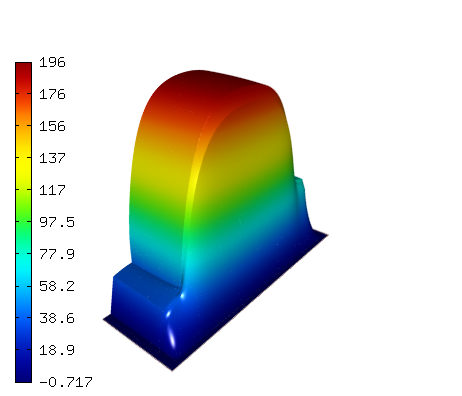
\includegraphics[height=5cm]{nist/nist-5/solution.png}
%\vspace{-3mm}
\caption{Solution to the NIST-5 benchmark problem.}
\label{fig:sln-nist05}
\end{figure}

Fig. \ref{fig:nist-5-hp-aniso} presents the final meshes corresponding to adaptive $h$-FEM with
linear elements, adaptive $h$-FEM with quadratic elements, and adaptive $hp$-FEM. Different
polynomial degrees of elements are represented by different colors.

\begin{figure}[H]
\centering
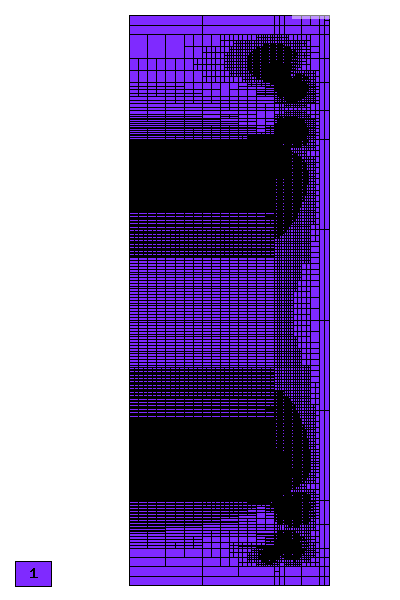
\includegraphics[height=5cm]{nist/nist-5/mesh_h1_aniso.png}
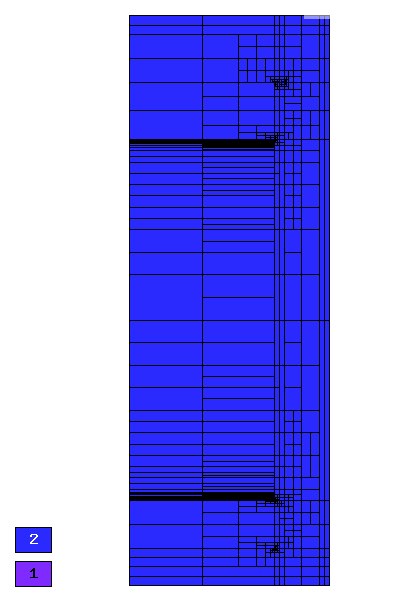
\includegraphics[height=5cm]{nist/nist-5/mesh_h2_aniso.png}
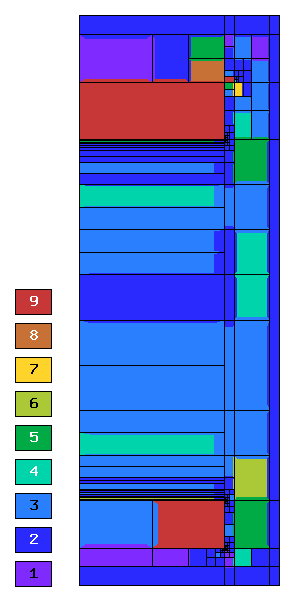
\includegraphics[height=5cm]{nist/nist-5/mesh_hp_aniso.png}
\caption{
Left: Final mesh with 55577 DOF and relative error 9.57345e-02~\% for $h$-FEM with linear elements.
Middle: Final mesh with 12483 DOF and relative error 1.34925e-02~\% for $h$-FEM with quadratic elements.
Right: Final mesh with 7450 DOF and relative error 1.46775e-02~\% for $hp$-FEM (adaptivity option HP\_ANISO\_H).}
\label{fig:nist-5-hp-aniso}
\end{figure}

Fig. \ref{fig:nist-5-conv} shows the convergence of the adaptive methods in terms of DOF and CPU-time.

\begin{figure}[H]
\centering
\hspace{-50mm}
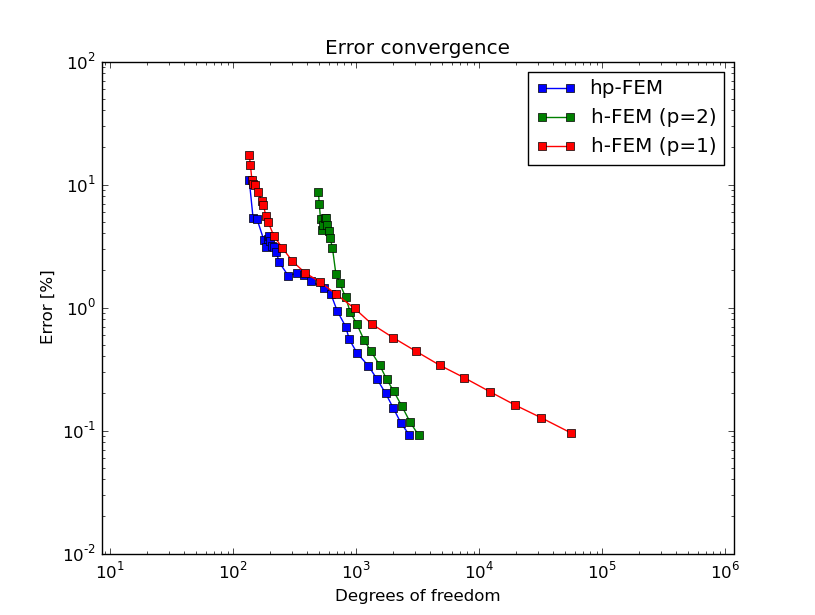
\includegraphics[width=7.5cm]{nist/nist-5/conv_dof_aniso.png}\ \
\hspace{-10mm}
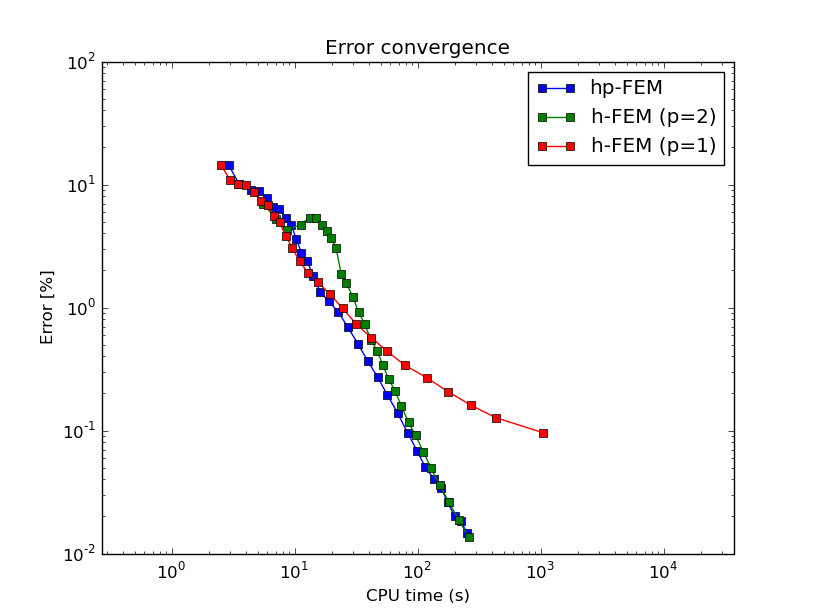
\includegraphics[width=7.5cm]{nist/nist-5/conv_cpu_aniso.png}
\hspace{-50mm}
\vspace{-2mm}
\caption{DOF and CPU time convergence graphs.}
\label{fig:nist-5-conv}
\end{figure}

%%%%%%%%%%%%%%%%%%%%%%%%%%%%%%%%%%%%%%%%%%%%%%%%

\section{Benchmark NIST-6 "Boundary Layer"}
\label{sec:bench-6}

This example is a singularly perturbed problem with known exact solution that exhibits
a boundary layer along the right and top sides of the domain.
It is a convection-diffusion equation with first order terms.

\begin{equation} \label{boundary-layer}
-\epsilon \nabla^{2} u + 2\frac{\partial u}{\partial x} + \frac{\partial u}{\partial y} = f
\end{equation}
in the domain $\Omega = (-1, 1)^2$, equipped with Dirichlet boundary condition
given by the exact solution. The exact solution is
$u(x,y) = (1 - e^{-(1 - x) / \epsilon})(1 - e^{-(1 - y) / \epsilon})cos(\pi (x + y))$,
where $\epsilon$ determines the strength of the boundary layer.
The solution to NIST-6 containing a boundary layer
with $\epsilon = 10^{-1}$ is shown in Fig. \ref{fig:sln-nist06}.

\begin{figure}[H]
\centering
\vspace{-3mm}
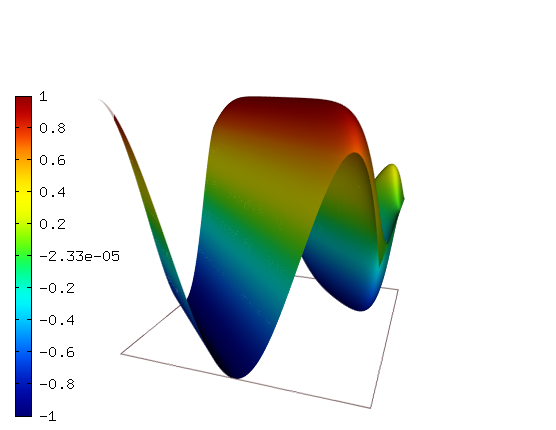
\includegraphics[height=5cm]{nist/nist-6/solution.png}
\caption{Solution to the NIST-6 benchmark problem.}
\vspace{-3mm}
\label{fig:sln-nist06}
\end{figure}

Fig. \ref{fig:nist-6-hp-aniso} presents the final meshes corresponding to adaptive $h$-FEM with
linear elements, adaptive $h$-FEM with quadratic elements, and adaptive $hp$-FEM. Different
polynomial degrees of elements are represented by different colors.

\begin{figure}[H]
\centering
%\vspace{-3mm}
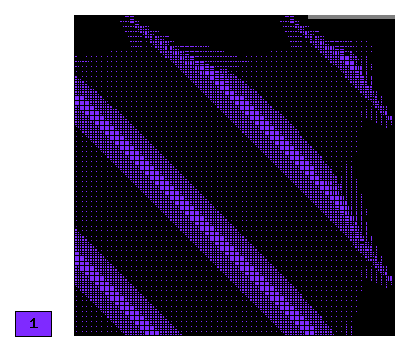
\includegraphics[height=3.7cm]{nist/nist-6/mesh_h1_aniso.png}
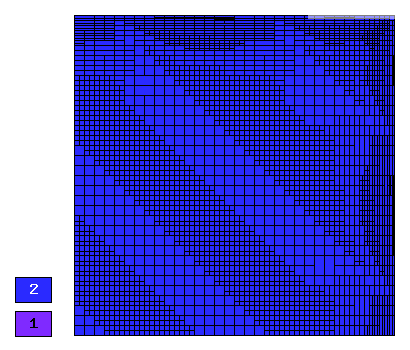
\includegraphics[height=3.7cm]{nist/nist-6/mesh_h2_aniso.png}
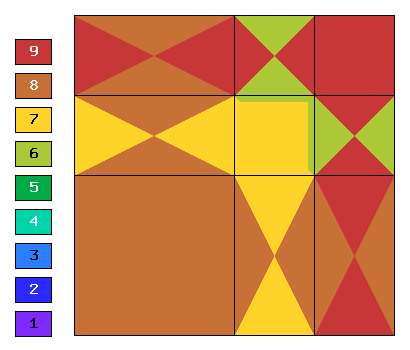
\includegraphics[height=3.7cm]{nist/nist-6/mesh_hp_aniso.png}
%\vspace{-3mm}
\caption{
Left: Final mesh with 55090 DOF and relative error 8.74769e-01~\% for $h$-FEM with linear elements.
Middle: Final mesh with 63145 DOF and relative error 1.46642e-02~\% for $h$-FEM with quadratic elements.
Right: Final mesh with 511 DOF and relative error 7.22919e-04~\% for $hp$-FEM (adaptivity option HP\_ANISO).}
\vspace{-2mm}
\label{fig:nist-6-hp-aniso}
\end{figure}

Fig. \ref{fig:nist-6-conv} shows the convergence of the adaptive methods in terms of DOF and CPU-time.

\begin{figure}[H]
\centering
%\vspace{-2mm}
\hspace{-50mm}
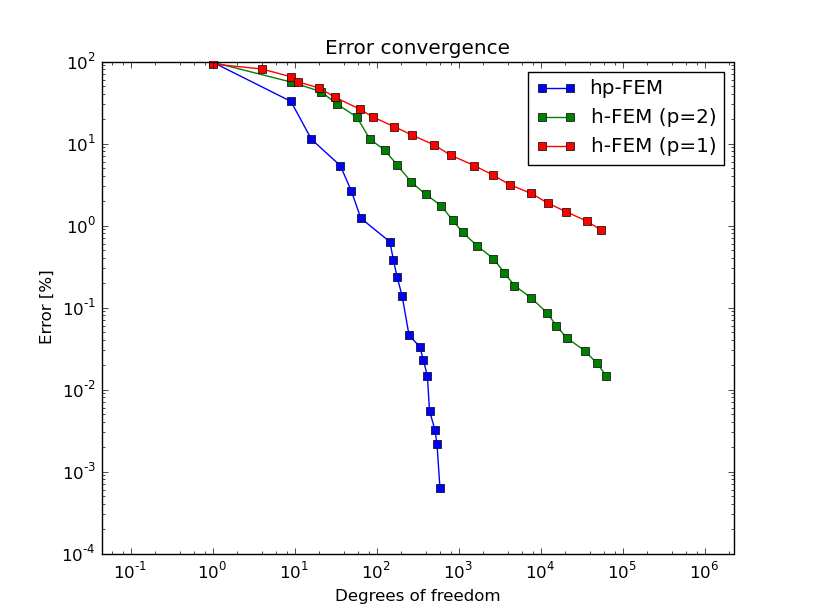
\includegraphics[width=7.5cm]{nist/nist-6/conv_dof_aniso.png}\ \
\hspace{-10mm}
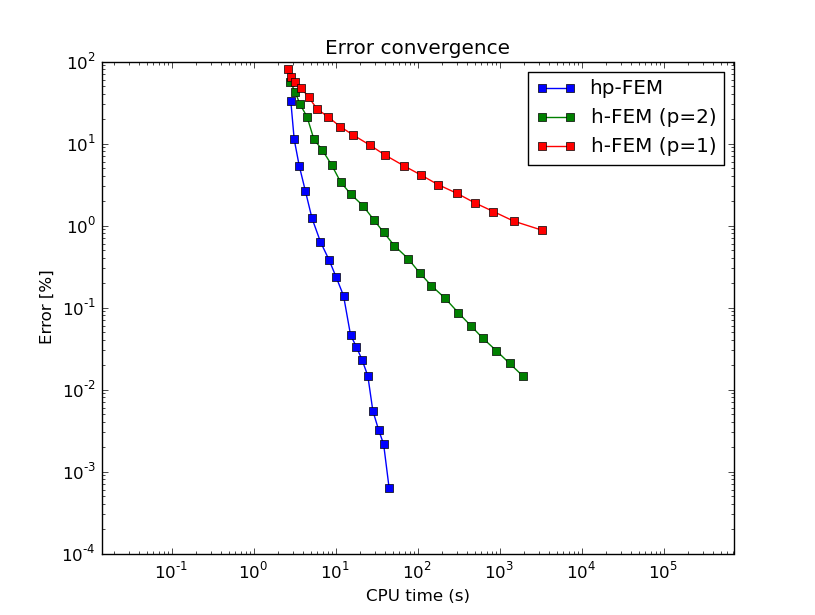
\includegraphics[width=7.5cm]{nist/nist-6/conv_cpu_aniso.png}
\hspace{-50mm}
\vspace{-2mm}
\caption{DOF and CPU time convergence graphs.}
\label{fig:nist-6-conv}
\end{figure}

%%%%%%%%%%%%%%%%%%%%%%%%%%%%%%%%%%%%%%%%%%%%%%%%

\section{Benchmark NIST-7 "Boundary Line Singularity"}
\label{sec:bench-7}

This is a singularity problem with the solution that is singular along the left part of the boundary.
The equation solved in this problem is the Poisson equation.

\begin{equation} \label{boundary-line-singularity}
-\Delta u = f
\end{equation}
in the domain $\Omega = (0, 1)^2$, equipped with Dirichlet boundary conditions
given by the exact solution. The exact solution is
$u(x,y) = x^{\alpha}$,
where $\alpha \geq 0.5$ determines the strength of the singularity.
The solution to NIST-7 with $\alpha = 0.6$ is shown in Fig. \ref{fig:sln-nist07}.

\begin{figure}[H]
\centering
%\vspace{-3mm}
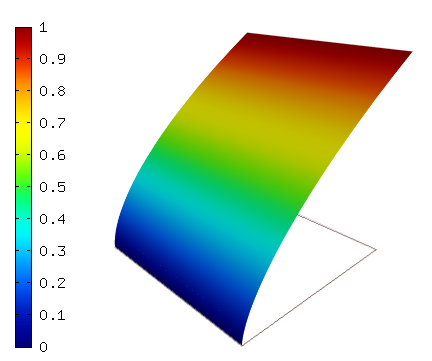
\includegraphics[height=5cm]{nist/nist-7/solution.png}
\vspace{-3mm}
\caption{Solution to the NIST-7 benchmark problem.}
%\vspace{-2mm}
\label{fig:sln-nist07}
\end{figure}

Fig. \ref{fig:nist-7-hp-aniso} presents the final meshes corresponding to adaptive $h$-FEM with
linear elements, adaptive $h$-FEM with quadratic elements, and adaptive $hp$-FEM. Different
polynomial degrees of elements are represented by different colors.

\begin{figure}[H]
\centering
%\vspace{-5mm}
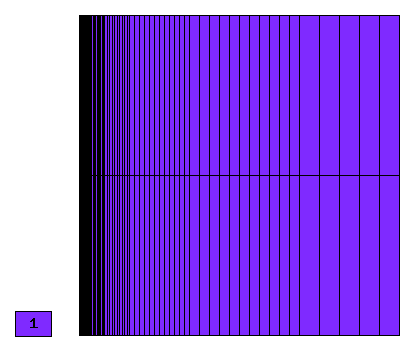
\includegraphics[height=3.7cm]{nist/nist-7/mesh_h1_aniso.png}
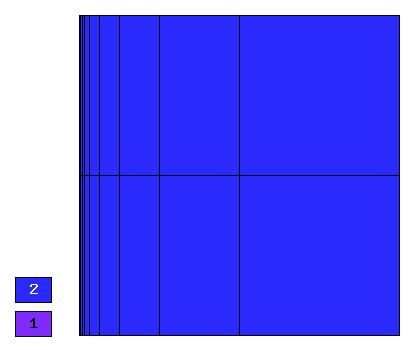
\includegraphics[height=3.7cm]{nist/nist-7/mesh_h2_aniso.png}
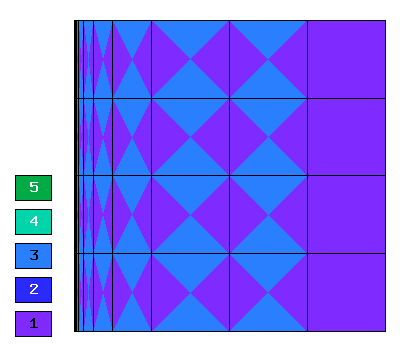
\includegraphics[height=3.7cm]{nist/nist-7/mesh_hp_aniso.png}
%\vspace{-3mm}
\caption{
Left: Final mesh with 684 DOF and relative error 1.45724~\% for $h$-FEM with linear elements.
Middle: Final mesh with 267 DOF and relative error 1.49585~\% for $h$-FEM with quadratic elements.
Right: Final mesh with 88 DOF and relative error 1.46348~\% for $hp$-FEM (adaptivity option HP\_ANISO\_H).}
%\vspace{-3mm}
\label{fig:nist-7-hp-aniso}
\end{figure}

Fig. \ref{fig:nist-7-conv} shows the convergence of the adaptive methods in terms of DOF and CPU-time.

\begin{figure}[H]
\centering
\hspace{-50mm}
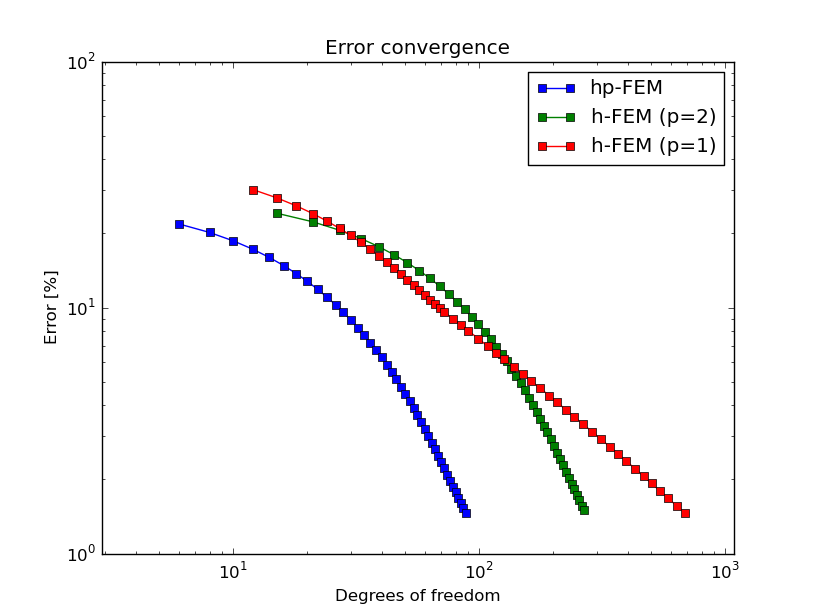
\includegraphics[width=7.5cm]{nist/nist-7/conv_dof_aniso.png}\ \
\hspace{-10mm}
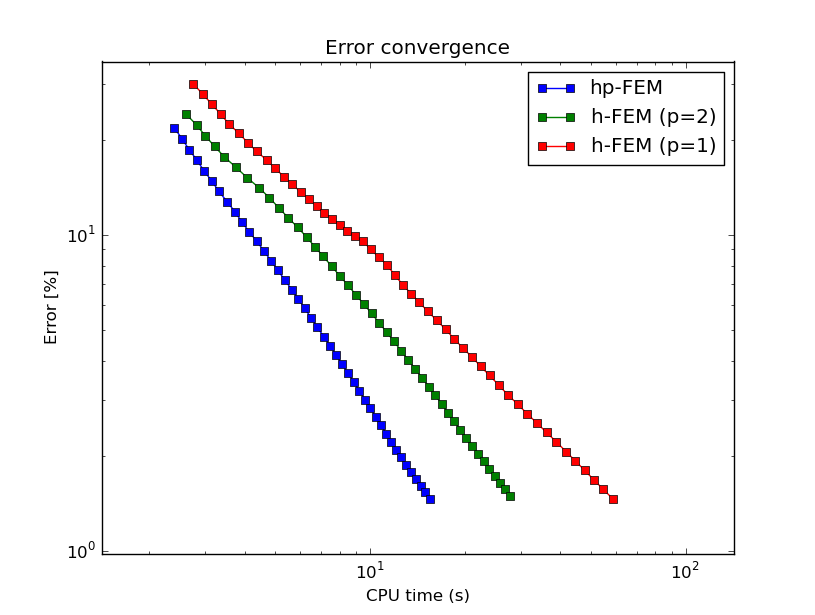
\includegraphics[width=7.5cm]{nist/nist-7/conv_cpu_aniso.png}
\hspace{-50mm}
\vspace{-2mm}
\caption{DOF and CPU time convergence graphs.}
\label{fig:nist-7-conv}
\end{figure}

%%%%%%%%%%%%%%%%%%%%%%%%%%%%%%%%%%%%%%%%%%%%%%%%

\section{Benchmark NIST-8 "Oscillatory"}
\label{sec:bench-8}

This is a wave function that satisfies the Schr\"{o}dinger's equation model of two
interacting atoms, highly oscillatory near the origin.
The equation solved in this problem is the Helmholtz equation.

\begin{equation} \label{oscillatory}
-\nabla^{2} u - \frac{1}{(\alpha + r)^{4}} u = f
\end{equation}
in the domain $\Omega = (0, 1)^2$, equipped with Dirichlet boundary conditions
given by the exact solution. The exact solution is
$u(x,y) = sin(\frac{1}{\alpha + r})$,
where $r = \sqrt{x^{2} + y^{2}}$, $\alpha = 1 / N \pi$ determines the number of oscillations.
The solution to NIST-8 with $\alpha = 1 / 10 \pi$ is shown in Fig. \ref{fig:sln-nist08}.

\begin{figure}[H]
\centering
\vspace{-3mm}
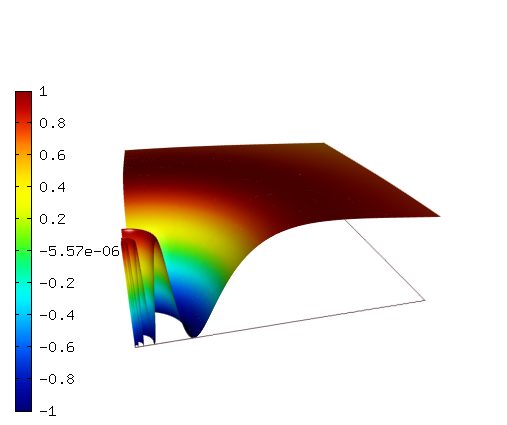
\includegraphics[height=5cm]{nist/nist-8/solution.png}
%\vspace{-3mm}
\caption{Solution to the NIST-8 benchmark problem.}
%\vspace{-4mm}
\label{fig:sln-nist08}
\end{figure}

Fig. \ref{fig:nist-8-hp-aniso} presents the final meshes corresponding to adaptive $h$-FEM with
linear elements, adaptive $h$-FEM with quadratic elements, and adaptive $hp$-FEM. Different
polynomial degrees of elements are represented by different colors.

\begin{figure}[H]
\centering
%\vspace{-5mm}
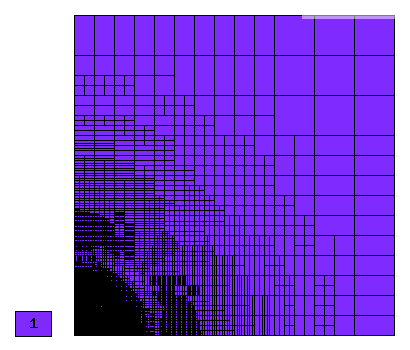
\includegraphics[height=3.7cm]{nist/nist-8/mesh_h1_aniso.png}
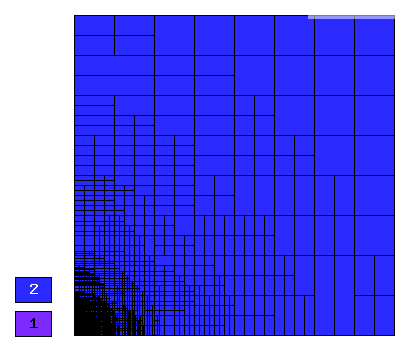
\includegraphics[height=3.7cm]{nist/nist-8/mesh_h2_aniso.png}
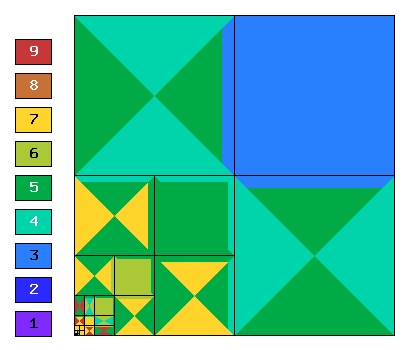
\includegraphics[height=3.7cm]{nist/nist-8/mesh_hp_aniso.png}
%\vspace{-3mm}
\caption{
Left: Final mesh with 55731 DOF and relative error 1.24198~\% for $h$-FEM with linear elements.
Middle: Final mesh with 28497 DOF and relative error 7.74787e-02~\% for $h$-FEM with quadratic elements.
Right: Final mesh with 1060 DOF and relative error 8.68330e-02~\% for $hp$-FEM (adaptivity option HP\_ANISO).}
%\vspace{-5mm}
\label{fig:nist-8-hp-aniso}
\end{figure}

Fig. \ref{fig:nist-8-conv} shows the convergence of the adaptive methods in terms of DOF and CPU-time.

\begin{figure}[H]
\centering
%\vspace{-4mm}
\hspace{-50mm}
\includegraphics[width=7.5cm]{nist/nist-8/conv_dof_aniso.png}\ \
\hspace{-10mm}
\includegraphics[width=7.5cm]{nist/nist-8/conv_cpu_aniso.png}
\hspace{-50mm}
\vspace{-2mm}
\caption{DOF and CPU time convergence graphs.}
\label{fig:nist-8-conv}
\end{figure}

%%%%%%%%%%%%%%%%%%%%%%%%%%%%%%%%%%%%%%%%%%%%%%%%

\section{Benchmark NIST-9 "Wave Front"}
\label{sec:bench-9}

This is a commonly used example for testing the performance of
adaptive refinement algorithms using a wave front and a singularity \cite{mitchell-1, mitchell-2}.
The solution has a sharp circular wave front in the interior of the
domain, with a singularity at the center of the circle.
The equation solved is the Poisson equation.

\begin{equation} \label{wave-front}
-\Delta u = f
\end{equation}
in the domain $\Omega = (0, 1)^2$, equipped with Dirichlet boundary conditions
given by the exact solution. The exact solution is
$u(x, y) = tan^{-1}(\alpha (r - r_{0}))$,
where $r = \sqrt{(x - x_{loc})^{2} + (y - y_{loc})^{2}}$.
Here $(x_{loc}, y_{loc})$ is the center of the circular wave front,
$r_{0}$ is the distance from the wave front to the center of the circle,
and $\alpha$ gives the steepness of the wave front.
The solution to NIST-9 with $\alpha = 50$, $(x_{loc}, y_{loc}) = (0.5, 0.5)$,
$r_{0} = 0.25$ is shown in Fig. \ref{fig:sln-nist09}.

\begin{figure}[H]
\centering
\vspace{-3mm}
\includegraphics[height=5cm]{nist/nist-9/solution.png}
\vspace{-1mm}
\caption{Solution to the NIST-9 benchmark problem.}
\vspace{-1mm}
\label{fig:sln-nist09}
\end{figure}

Fig. \ref{fig:nist-9-hp-aniso} presents the final meshes corresponding to adaptive $h$-FEM with
linear elements, adaptive $h$-FEM with quadratic elements, and adaptive $hp$-FEM. Different
polynomial degrees of elements are represented by different colors.

\begin{figure}[H]
\centering
%\vspace{-5mm}
\includegraphics[height=3.7cm]{nist/nist-9/mesh_h1_aniso.png}
\includegraphics[height=3.7cm]{nist/nist-9/mesh_h2_aniso.png}
\includegraphics[height=3.7cm]{nist/nist-9/mesh_hp_aniso.png}
%\vspace{-5mm}
\caption{
Left: Final mesh with 46093 DOF and relative error 1.23973~\% for $h$-FEM with linear elements.
Middle: Final mesh with 36849 DOF and relative error 7.80979e-02~\% for $h$-FEM with quadratic elements.
Right: Final mesh with 2781 DOF and relative error 7.54155e-02~\% for $hp$-FEM (adaptivity option HP\_ANISO).}
\vspace{-5mm}
\label{fig:nist-9-hp-aniso}
\end{figure}

Fig. \ref{fig:nist-9-conv} shows the convergence of the adaptive methods in terms of DOF and CPU-time.

\begin{figure}[H]
\centering
%\vspace{-3mm}
\hspace{-50mm}
\includegraphics[width=7.5cm]{nist/nist-9/conv_dof_aniso.png}\ \
\hspace{-10mm}
\includegraphics[width=7.5cm]{nist/nist-9/conv_cpu_aniso.png}
\hspace{-50mm}
\vspace{-2mm}
\caption{DOF and CPU time convergence graphs.}
\label{fig:nist-9-conv}
\end{figure}

%%%%%%%%%%%%%%%%%%%%%%%%%%%%%%%%%%%%%%%%%%%%%%%%

\section{Benchmark NIST-10 "Interior Line Singularity"}
\label{sec:bench-10}

This is another example with anisotropic solution that is suitable for testing
anisotropic element refinements. The equation solved is the Poisson equation.
\begin{equation} \label{interior}
-\Delta u = f
\end{equation}
in the domain $\Omega = (-1, 1)^2$, equipped with a zero
Neumann boundary condition on left edge, Dirichlet boundary
conditions given by the exact solution on the rest of the boundary.
The exact solution is
$u(x,y) = \cos(Ky)\ (x \le 0)$ and $u(x,y) = \cos(Ky) + x^{\alpha}\ (x > 0)$,
where $K$ and $\alpha$ are constants.
The solution to NIST-10 containing a line singularity with $K = \pi/2$ and
$\alpha = 2.01$ is shown in Fig. \ref{fig:sln-nist10}.

\begin{figure}[H]
\centering
\vspace{-6mm}
\includegraphics[height=5cm]{nist/nist-10/solution.png}
\vspace{-3mm}
\caption{Solution to the NIST-10 benchmark problem.}
\vspace{-3mm}
\label{fig:sln-nist10}
\end{figure}

Fig. \ref{fig:nist-10-hp-aniso} presents the final meshes corresponding to adaptive $h$-FEM with
linear elements, adaptive $h$-FEM with quadratic elements, and adaptive $hp$-FEM. Different
polynomial degrees of elements are represented by different colors.

\begin{figure}[H]
\centering
%\vspace{-3mm}
\includegraphics[height=3.7cm]{nist/nist-10/mesh_h1_aniso.png}
\includegraphics[height=3.7cm]{nist/nist-10/mesh_h2_aniso.png}
\includegraphics[height=3.7cm]{nist/nist-10/mesh_hp_aniso.png}
%\vspace{-3mm}
\caption{
Left: Final mesh with 27999 DOF and relative error 2.87268e-01~\% for $h$-FEM with linear elements.
Middle: Final mesh with 60144 DOF and relative error 2.59816e-04~\% for $h$-FEM with quadratic elements.
Right: Final mesh with 147 DOF and relative error 9.01829e-05~\% for $hp$-FEM (adaptivity option HP\_ANISO).}
%\vspace{-3mm}
\label{fig:nist-10-hp-aniso}
\end{figure}

Fig. \ref{fig:nist-10-conv} shows the convergence of the adaptive methods in terms of DOF and CPU-time.

\begin{figure}[H]
\centering
%\vspace{-3mm}
\hspace{-50mm}
\includegraphics[width=7.5cm]{nist/nist-10/conv_dof_aniso.png}\ \
\hspace{-10mm}
\includegraphics[width=7.5cm]{nist/nist-10/conv_cpu_aniso.png}
\hspace{-50mm}
\vspace{-2mm}
\caption{DOF and CPU time convergence graphs.}
\label{fig:nist-10-conv}
\end{figure}

%%%%%%%%%%%%%%%%%%%%%%%%%%%%%%%%%%%%%%%%%%%%%%%%

\section{Benchmark NIST-11 "Intersecting Interfaces"}
\label{sec:bench-11}

This is a Poisson problem with intersecting interfaces,
dividing the plane into four regions.
The solution to this problem contains a severe
singularity that poses a challenge to adaptive methods.
The equation solved is given by

\begin{equation} \label{intersecting}
-\nabla \cdot (a(x,y) \nabla u) = 0
\end{equation}
where the parameter $a$ is piecewise-constant,
$a(x,y) = 161.4476387975881$ in the first and third quadrants,
and $a(x,y) = 1$ in the remaining two quadrants.
The domain of this problem is $\Omega = (-1, 1)^2$, equipped with
Dirichlet boundary conditions given by the exact solution.
The exact solution is
$u(x,y) = r^{a_1} \mu (\theta)$,
where $a_1$ and $\mu (\theta)$ is given in \cite{mitchell-1}.
The solution to NIST-11 is shown in Fig. \ref{fig:sln-nist11}.

\begin{figure}[H]
\centering
%\vspace{-5mm}
\includegraphics[height=4.7cm]{nist/nist-11/solution.png}
%\vspace{-2mm}
\caption{Solution to the NIST-11 benchmark problem.}
%\vspace{-3mm}
\label{fig:sln-nist11}
\end{figure}

Fig. \ref{fig:nist-11-hp-aniso} presents the final meshes corresponding to adaptive $h$-FEM with
linear elements, adaptive $h$-FEM with quadratic elements, and adaptive $hp$-FEM. Different
polynomial degrees of elements are represented by different colors.

\begin{figure}[H]
\centering
%\vspace{-2mm}
\includegraphics[height=3.7cm]{nist/nist-11/mesh_h1_aniso.png}
\includegraphics[height=3.7cm]{nist/nist-11/mesh_h2_aniso.png}
\includegraphics[height=3.7cm]{nist/nist-11/mesh_hp_aniso.png}
%\vspace{-3mm}
\caption{
Left: Final mesh with 46905 DOF and relative error 1.25659~\% for $h$-FEM with linear elements.
Middle: Final mesh with 7777 DOF and relative error 4.73604e-01~\% for $h$-FEM with quadratic elements.
Right: Final mesh with 3459 DOF and relative error 4.7087e-01~\% for $hp$-FEM (adaptivity option HP\_ANISO\_H).}
%\vspace{-2mm}
\label{fig:nist-11-hp-aniso}
\end{figure}

Fig. \ref{fig:nist-11-conv} shows the convergence of the adaptive methods in terms of DOF and CPU-time.

\begin{figure}[H]
\centering
\hspace{-50mm}
\includegraphics[width=7.5cm]{nist/nist-11/conv_dof_aniso.png}\ \
\hspace{-10mm}
\includegraphics[width=7.5cm]{nist/nist-11/conv_cpu_aniso.png}
\hspace{-50mm}
\vspace{-2mm}
\caption{DOF and CPU time convergence graphs.}
\label{fig:nist-11-conv}
\end{figure}

%%%%%%%%%%%%%%%%%%%%%%%%%%%%%%%%%%%%%%%%%%%%%%%%

\section{Benchmark NIST-12 "Multiple Difficulties"}
\label{sec:bench-12}

This problem combines four aspects of benchmarks
seen in previous sections (nist-2, nist-4, nist-6 and nist-9) into one problem.
The wave front intersects the boundary
layer and corner singularity, and the peak is centered on the wave front.
The equation solved is the Poisson equation.
\begin{equation} \label{multiple}
-\Delta u = f
\end{equation}
in the L-shaped domain, equipped with Dirichlet boundary conditions
given by the exact solution.
The exact solution is

\[
u(x,y) =  r^{\alpha_{C} }\sin(\alpha_{C} \theta)
+ e^{-\alpha_{P} ((x - x_{P})^{2} + (y - y_{P})^{2})}
+ e^{-(1 + y) / \epsilon}
+ tan^{-1}(\alpha_{W} (r_{W} - r_{0}))
\]
where $\alpha_C = \pi / \omega_C$, $r = \sqrt{x^2+y^2}$
and $\theta = tan^{-1}(y/x)$, here $\omega_C$ determines
the angle of the re-entrant corner.
$(x_{P}, y_{P})$ is the location of the peak, $\alpha_{P}$
determines the strength of the peak.
The parameter $\epsilon$ determines the
strength of the boundary layer, the boundary layer was placed on $y = -1$.
Furthermore
$r_{W} = \sqrt{(x - x_{W})^{2} + (y - y_{W})^{2}}$,
where $(x_{W}, y_{W})$ is the center of the circular wave front,
$r_{0}$ is the distance from the wave front to the
center of the circle, and $\alpha_W$ gives
the steepness of the wave front.
The solution to NIST-12 with $\omega_C = 3 \pi /2$,
$\alpha_{P} = 1000$, $(x_{P}, y_{P}) = (\sqrt{5} / 4, -1/4)$,
$\epsilon = 1/100$,
$\alpha_{W} = 200$, $(x_{W}, y_{W}) = (0, -3/4)$, $r_{0} = 3/4$
is shown in Fig. \ref{fig:sln-nist12}.

\begin{figure}[H]
\centering
\includegraphics[height=5cm]{nist/nist-12/solution.png}
\caption{Solution to the NIST-12 benchmark problem.}
\label{fig:sln-nist12}
\end{figure}

Fig. \ref{fig:nist-12-hp-aniso} presents the final meshes corresponding to adaptive $h$-FEM with
linear elements, adaptive $h$-FEM with quadratic elements, and adaptive $hp$-FEM. Different
polynomial degrees of elements are represented by different colors.

\begin{figure}[H]
\centering
\includegraphics[height=3.7cm]{nist/nist-12/mesh_h1_aniso.png}
\includegraphics[height=3.7cm]{nist/nist-12/mesh_h2_aniso.png}
\includegraphics[height=3.7cm]{nist/nist-12/mesh_hp_aniso.png}
\caption{
Left: Final mesh with 45533 DOF and relative error 2.05698~\% for $h$-FEM with linear elements.
Middle: Final mesh with 56975 DOF and relative error 1.54977e-01~\% for $h$-FEM with quadratic elements.
Right: Final mesh with 9162 DOF and relative error 9.65869e-02~\% for $hp$-FEM (adaptivity option HP\_ANISO).}
\label{fig:nist-12-hp-aniso}
\end{figure}

Fig. \ref{fig:nist-12-conv} shows the convergence of the adaptive methods in terms of DOF and CPU-time.

\begin{figure}[H]
\centering
\hspace{-50mm}
\includegraphics[width=7.5cm]{nist/nist-12/conv_dof_aniso.png}\ \
\hspace{-10mm}
\includegraphics[width=7.5cm]{nist/nist-12/conv_cpu_aniso.png}
\hspace{-50mm}
\vspace{-2mm}
\caption{DOF and CPU time convergence graphs.}
\label{fig:nist-12-conv}
\end{figure}
%\vspace{-8mm}
%%%%%%%%%%%%%%%%%%%%%%%%%%%%%%%%%%%%%%%%%%%%%%%%%%%%%%%

\section{Conclusion and Outlook}
\label{sec:conclusion}

We solved a suite of twelve benchmark problems from \cite{mitchell-1}
using an open-source finite library Hermes. The numerical results are
easily reproducible as they are part of the Git repository of the
open source project. More information about the Hermes library can be found
in an extensive User Documentation that is available on the project home
page http://hpfem.org/hermes/. In particular, these 12 examples are located
in the directory hermes/hermes2d/ benchmarks/.

\section{Acknowledgment}

This work was supported by Subcontract No. 00089911 of Battelle
Energy Alliance (DOE intermediary) as well as by the
Grant No. IAA100760702 of the Grant Agency of the Academy
of Sciences of the Czech Republic. The first autor was partly
supported by the National Natural Science Foundation
of China under Projects No. 41074099.

%\noindent

%% Authors are advised to submit their bibtex database files. They are
%% requested to list a bibtex style file in the manuscript if they do
%% not want to use elsarticle-num.bst.

%% References without bibTeX database:

% \begin{thebibliography}{00}	

%% \bibitem must have the following form:
%%   \bibitem{key}...
%%

% \bibitem{}

% \end{thebibliography}

\begin{thebibliography}{[KLR73]}

\bibitem{mitchell-1}
W. Mitchell: A Collection of 2D Elliptic Problems for
Testing Adaptive Algorithms, NISTIR 7668, 2010 (available online).

\vspace{-2mm}

\bibitem{mitchell-2}
W. Mitchell: A Survey of hp-Adaptive Strategies for Elliptic Partial Differential Equations,
Annals of the European Academy of Sciences, to appear (available online).

\vspace{-2mm}

%\bibitem{demkowicz-1}
%L. Demkowicz: One and Two Dimensional Elliptic and Maxwell Problems,
%Chapman \& Hall \/ CRC Press, Taylor \& Francis, 2006.


\bibitem{label2}
P. Solin, D. Andrs, J. Cerveny, M. Simko:
PDE-Independent Adaptive $hp$-FEM Based on Hierarchic Extension of Finite Element Spaces.
J. Comput. Appl. Math. 233 (2010) 3086-3094.

\vspace{-2mm}

\bibitem{thermoel}
P. Solin, J. Cerveny, L. Dubcova, D. Andrs:
Monolithic Discretization of Linear Thermoelasticity Problems
via Adaptive Multimesh $hp$-FEM, J. Comput. Appl. Math 234 (2010) 2350 - 2357.

\vspace{-2mm}

\bibitem{sosedo}
P. Solin. K. Segeth, I. Dolezel: Higher-Order Finite Element Methods, Chapman \& Hall
/ CRC Press, Boca Raton, 2003.
\end{thebibliography}

%\newpage

\end{document}

%%
%% End of file `elsarticle-template-num.tex'.
